\documentclass[11pt]{article}

\usepackage[margin=1in]{geometry}
\usepackage{amsmath,amssymb}
\usepackage{graphicx}
\usepackage{booktabs}
\usepackage{natbib}
\usepackage[hidelinks]{hyperref}
\usepackage{xcolor}
\usepackage{caption}

\captionsetup{font=small,labelfont=bf}
\graphicspath{{figures/}}

\title{\textbf{When Should an NHL Team Pull Its Goalie?}\\[2pt]
\large A Reproducible Bayesian Decision-Analysis Workflow\\ on Modern Play-by-Play Data}

\author{Adriana-Stefania Ciupeanu\thanks{Correspondence: \texttt{cadrianas@gmail.com}.
Code and data: \url{https://github.com/cadrianas/nhl-goalie-pull}.}}

\date{\today}

\begin{document}
\maketitle

\begin{abstract}
\noindent
Pulling the goalie for an extra attacker is the canonical in-game decision in
hockey: a trailing team trades a higher chance of scoring for a higher chance of
conceding an empty-net goal. We present an end-to-end, reproducible Bayesian
decision-analysis of this problem on three recent seasons (2022--2024) of
National Hockey League (NHL) play-by-play. The
workflow combines two public data sources---shot-level data with pre-computed
expected goals and the NHL's play-by-play feed---to recover both the goal
\emph{events} and the continuous \emph{exposure time} needed to estimate rates,
and it separates genuine late trailing pulls from the delayed-penalty empty nets
that otherwise contaminate them. Goal rates are modeled with conjugate
Gamma--Poisson posteriors and fed through a backward-induction optimal-stopping
solver whose terminal value is expected standings points. Carrying the full
posterior through the solver yields a \emph{distribution} over the optimal pull
time. We find that the expected-points-optimal pull time when trailing by one
goal is roughly $6$:$44$ of regulation remaining---far earlier than the observed
coaching median of about $2$:$00$---and that pulling optimally is worth on the
order of half a standings point per team per season. Two refinements sharpen the
picture without overturning it: a hierarchical model shows that team and opponent
effects on the pulled rates are small, so the optimal pull time is nearly
universal (a \emph{decision} problem, not a \emph{talent} problem); and a
time-inhomogeneous hazard model documents that the trailing team's even-strength
scoring rate collapses over the final minutes---violating the constant-rate
assumption common in prior work---yet shifts the optimum by only seconds. The
aggressive-pull prescription is thus robust to each refinement. All code, a
precomputed rate table, and an interactive decision tool are released.
\end{abstract}

\section{Introduction}

When an ice-hockey team trails late in a game, its coach may replace the goaltender
with an additional skater, creating a six-on-five attacking advantage at the cost
of an undefended net. The decision is a textbook problem in sequential
decision-making under uncertainty: pulling raises the rate at which the trailing
team scores, but also the rate at which it concedes, and conceding an empty-net
goal is close to terminal. The coach must choose \emph{when} to accept this
trade, as a function of the score and the time remaining.

The problem has a long analytical history. \citet{morrison1976optimal} introduced
a Poisson model but compared pulling at a single fixed time against never pulling;
\citet{morrison1986pulling} and \citet{washburn1991still} refined the
optimal-timing analysis, and \citet{beaudoin2010strategies} built a full-game
simulator with scoring rates estimated by constrained Bayesian methods, concluding
that coaches pull too conservatively---a trailing team should often pull with about
three minutes remaining. \citet{buttrey2011estimating} estimated NHL scoring rates
with an eye toward such decisions, and in widely-circulated work
\citet{brown2018pulling} argued, using a stochastic optimal-control model and the
insight that the relevant objective is expected \emph{standings points} rather than
expected goals, that teams should pull dramatically earlier still.

Our contribution is not a new estimator or a new theorem. It is a transparent,
reproducible \emph{workflow} that (i) assembles the two public data sources needed
to estimate the competing goal rates \emph{and} their exposure denominators;
(ii) handles a data confound---delayed-penalty empty nets---that is easy to
overlook; (iii) carries full Bayesian posterior uncertainty into an
optimal-stopping solver and therefore reports a distribution over the optimal pull
time; and (iv) stress-tests the conclusion against a hierarchical team model and a
time-inhomogeneous hazard model. In the spirit of ``modelling with data,'' we
release the complete pipeline, a precomputed rate table, and an interactive tool.
Several of our findings are deliberately negative---team identity barely moves the
answer; time-varying hazards barely move the answer---and we argue that this
robustness is itself the most useful result for a practitioner.

\section{Data}
\label{sec:data}

\paragraph{Sources.} We use two public feeds. MoneyPuck \citep{moneypuck} provides
one shot-level record per unblocked shot attempt, with the on-ice state (skaters
per side, empty-net flags), the score before the shot, and a pre-computed expected
goals (xG) value. The NHL play-by-play API \citep{nhlapi} provides every game
event with a \texttt{situationCode}---a four-digit encoding of which goaltenders
and how many skaters are on the ice---from which the continuous timeline of on-ice
states can be reconstructed. The shot feed supplies the \emph{events} (the
numerators of goal rates); the play-by-play supplies the \emph{exposure time} (the
denominators). Deriving both from play-by-play keeps numerator and denominator
mutually consistent.

\paragraph{Exposure reconstruction.} A rate requires time at risk, which shot data
alone cannot provide. For each game with a trailing pull we walk the play-by-play,
convert each \texttt{situationCode} into (empty-net team, skater counts), and treat
the interval between consecutive events as time spent in that state, tracking the
running score from goal events. Summing interval durations by game-state yields the
exposure denominators; goals scored within a state supply the numerators.

\paragraph{A confound: not every empty net is a goalie pull.} Teams also pull the
goaltender for a sixth attacker during a \emph{delayed penalty}, which can occur at
any time and at any score. Treating these as trailing pulls biases the rate
estimates. We therefore label a state a genuine \emph{late trailing pull} only when
the net is empty, the pulling team is behind, and the game is in regulation; this
removes roughly one in nine empty-net shots in our window. All downstream rates use
the filtered definition.

\paragraph{Scope.} We analyze regular-season games from the 2022, 2023, and 2024
seasons (season labeled by starting year), comprising about $3.6\times10^5$ shot
records and roughly $2{,}400$ games containing a trailing pull. The pipeline is
written to ingest additional seasons without modification.

\section{Methods}

\subsection{Competing goal rates}

While the goalie is pulled, goals arrive as two competing processes: goals
\emph{for} the trailing team (narrowing the deficit) at per-second rate
$\lambda^{\mathrm{out}}_{\mathrm{for}}$ and goals \emph{against} (into the empty
net) at rate $\lambda^{\mathrm{out}}_{\mathrm{against}}$. The counterfactual of
\emph{not} pulling has its own even-strength rates
$\lambda^{\mathrm{in}}_{\mathrm{for}},\lambda^{\mathrm{in}}_{\mathrm{against}}$.
Each rate is estimated per deficit $d\in\{1,2,3\}$ with a conjugate Gamma--Poisson
model: with a weakly-informative $\mathrm{Gamma}(\alpha_0,\beta_0)$ prior
(expressed as a small number of prior goals over prior seconds) and $g$ observed
goals over exposure $E$, the posterior is
\[
\lambda \mid g, E \;\sim\; \mathrm{Gamma}(\alpha_0 + g,\ \beta_0 + E).
\]
With hundreds of events per cell the prior is immaterial; the point of the Bayesian
treatment is that the full posterior is propagated into the decision.

\subsection{The decision: non-homogeneous optimal stopping}

Let the state be the signed deficit $d$ (positive: trailing) and the seconds
remaining $t$. Each second, under the chosen action's rates, the trailing team
scores (move to $d-1$), concedes (move to $d+1$), or neither. We solve by backward
induction on a one-second grid. The terminal value is \emph{expected standings
points}: a regulation win (reaching $d<0$) is worth $2$, reaching overtime tied
($d=0$) is worth $1.5$ (one guaranteed point plus a fair overtime coin flip), and a
regulation loss is worth $0$. This objective, following \citet{brown2018pulling},
is what makes pulling attractive: once a team is trailing, conceding another goal
costs little in points, while scoring to tie is worth a great deal. Modeling the
value over a signed-deficit grid---rather than stopping at the first tie---is what
distinguishes the points objective from a simpler probability-of-tying objective,
which merely rescales it.

The optimal policy is a threshold: pull when the time remaining first falls to
$t^\star_d$. Because we solve the recursion separately for each of several thousand
posterior draws of the rates, the output is a posterior distribution over
$t^\star_d$, from which we report the median and a $90\%$ credible interval. We
also evaluate the expected points of \emph{fixed} pull policies, which lets us
score a coach's actual timing against the optimum.

\subsection{Two refinements}

\paragraph{Hierarchical rates.} To ask whether the optimal timing depends on
\emph{who} is playing, we replace the pooled pulled rates with a hierarchical
Poisson model (fit in PyMC; \citealp{abrilpla2023pymc,kumar2019arviz}) with a log
link and partially-pooled, non-centered team effects for six-on-five attack and
suppression and for empty-net finishing and prevention, with per-deficit fixed
intercepts. The matchup-specific posterior rates feed the same solver unchanged.

\paragraph{Time-inhomogeneous hazards.} The constant-rate assumption is
questionable for the goalie-in counterfactual. We model the goalie-in for/against
hazards as smooth functions of time remaining---$\log\lambda[d,t] =
\text{level}[d] + \text{shape}(t)$ with $\text{shape}(t)$ a Gaussian random walk
over sixty-second bins---and extend the solver to use time-varying rates, turning
it into a non-homogeneous optimal-stopping problem.

\section{Results}

\subsection{Coaches pull far too late}

Table~\ref{tab:main} and Figure~\ref{fig:optimal} give the central result. Under
the expected-points objective, the optimal pull time when trailing by one is about
$404$ seconds ($6$:$44$) of regulation remaining, against an observed coaching
median of $119$ seconds ($1$:$59$). The gap narrows but persists at larger
deficits. Pulling optimally rather than never raises expected points from $0.27$
to $0.46$ when down one---a gain of about $0.19$ points per situation---and the
credible intervals on the optimal time are wide enough to be worth reporting but
nowhere near the observed behavior.

\begin{table}[t]
\centering
\caption{Optimal versus actual goalie-pull time, 2022--2024. ``Optimal'' is the
posterior-median expected-points threshold (90\% credible interval); ``actual'' is
the observed coaching median. Gain is the expected standings points added by
pulling optimally rather than never.}
\label{tab:main}
\begin{tabular}{lcccc}
\toprule
Deficit & Optimal pull (s rem.) & 90\% CI & Actual median & E[points] gain \\
\midrule
Down 1 & 404 (6:44) & 342--498 & 119 (1:59) & $+0.189$ \\
Down 2 & 394 (6:34) & 339--459 & 163 (2:43) & $+0.096$ \\
Down 3 & 377 (6:17) & 304--462 & 252 (4:12) & $+0.039$ \\
\bottomrule
\end{tabular}
\end{table}

\begin{figure}[t]
\centering
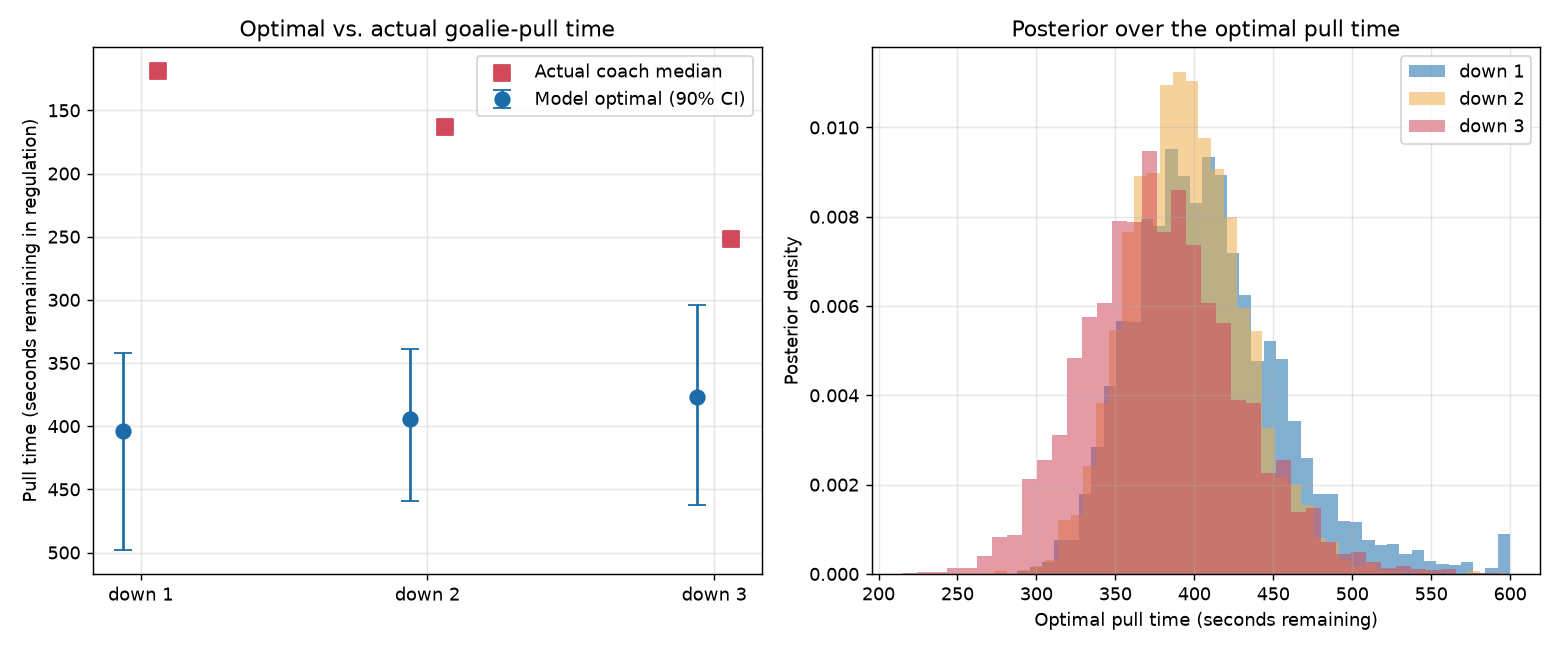
\includegraphics[width=0.95\textwidth]{optimal_pull_times.png}
\caption{Left: model-optimal pull time (blue, with 90\% credible interval) versus
observed coaching median (red), by deficit; higher is earlier. Right: the
posterior distribution over the optimal pull time.}
\label{fig:optimal}
\end{figure}

\subsection{The cost of conservatism, by team}

Scoring each team's actual pull timing against the optimum, from a common
down-by-one state, the average team forgoes about $0.54$ expected standings points
per season through late pulls (Figure~\ref{fig:cost}). The most conservative team
in the window (Nashville) leaves about $0.87$; the least (Toronto, Boston) about
$0.29$. Crucially, this total conflates \emph{decision quality} with
\emph{exposure}: a strong team can appear efficient simply by rarely trailing.
Separating the two motivates the hierarchical analysis.

\begin{figure}[t]
\centering
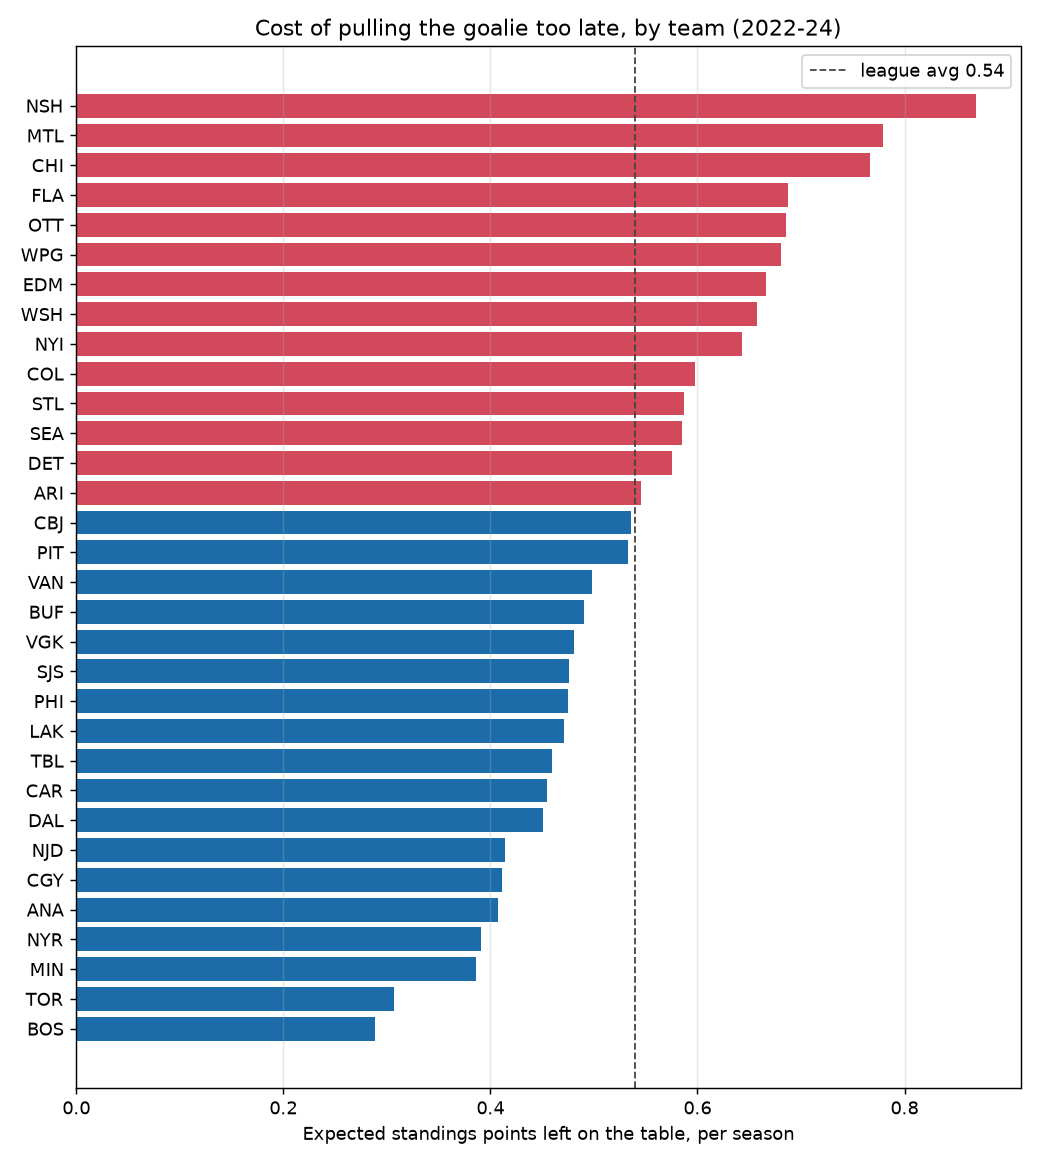
\includegraphics[width=0.72\textwidth]{points_left_by_team.png}
\caption{Expected standings points forgone per season by pulling later than
optimal, by team (red above the league average, blue below).}
\label{fig:cost}
\end{figure}

\subsection{It is a decision problem, not a talent problem}

The hierarchical model converges cleanly (maximum $\hat{R}=1.004$). After partial
pooling, team-to-team variation in the pulled rates is small: six-on-five for-rates
span only $0.141$--$0.151$ goals per sixty seconds and empty-net against-rates
$0.359$--$0.385$, about $\pm7\%$ around the mean. Propagated through the solver,
the team-specific optimal pull times cluster tightly---a down-one standard
deviation of roughly $28$ seconds across teams---around the league value
(Figure~\ref{fig:hier}). This spread is dwarfed by the $\sim\!350$-second gap
between the optimum and actual behavior. Teams are not meaningfully better or worse
at six-on-five play on the time scale that matters here; they are uniformly late.
The variation in points left on the table is therefore driven by how often a team
trails and by its timing choices, not by personnel.

\begin{figure}[t]
\centering
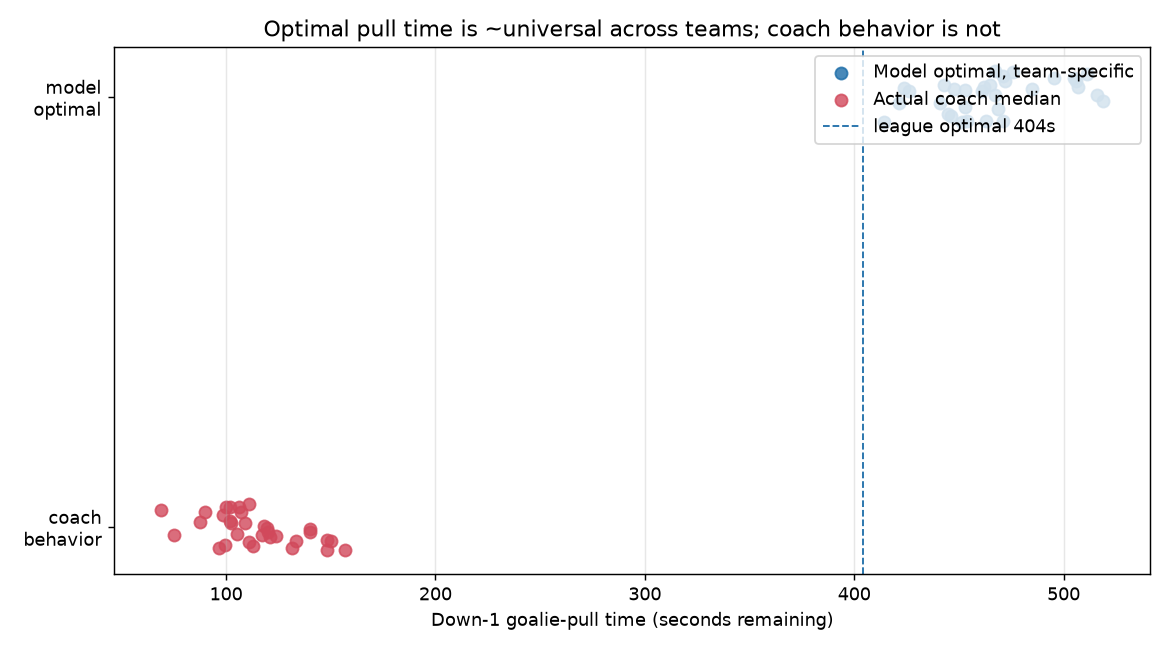
\includegraphics[width=0.85\textwidth]{hier_team_optima.png}
\caption{Team-specific optimal pull times (top) cluster tightly, while observed
coaching medians (bottom) sit far later. Personnel barely moves the optimum.}
\label{fig:hier}
\end{figure}

\subsection{Time-varying hazards: a wrong assumption, a small effect}

The trailing team's even-strength scoring rate is strongly time-inhomogeneous
(Figure~\ref{fig:hazard}): it rises through mid-period and then collapses over the
final roughly seven minutes---from about $0.044$ goals per sixty seconds across the
game to under $0.015$ late---so the constant period-three average over-prices the
offense available in the decision window. This directly violates the constant-rate
assumption common in prior treatments. Yet when the hazard shape is modeled and the
solver made non-homogeneous (maximum $\hat{R}=1.007$), the optimal pull time moves
by only $+12$ to $+25$ seconds. The decision is a genuinely non-homogeneous
optimal-stopping problem, but the aggressive-pull conclusion survives the
correction.

\begin{figure}[t]
\centering
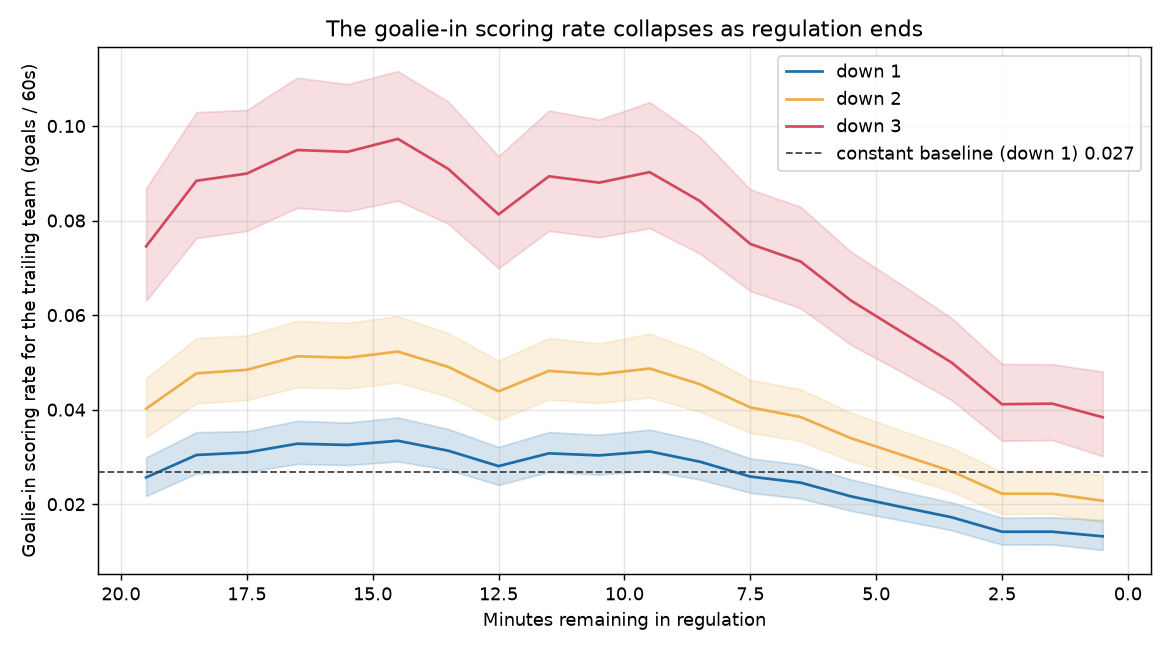
\includegraphics[width=0.85\textwidth]{goalie_in_hazard.png}
\caption{The trailing team's goalie-in scoring rate as a function of time
remaining, by deficit (posterior median and 90\% band). It collapses over the final
minutes, crossing below the constant baseline (dashed) used in prior work.}
\label{fig:hazard}
\end{figure}

\subsection{Out-of-sample validation}

Fitting the rates on 2022--2023 and checking the held-out 2024 season, all twelve
rate cells have observed goal counts inside their $95\%$ posterior-predictive
(Negative-Binomial) intervals, indicating no systematic miscalibration. The
recommended thresholds are also stable across the training and full samples (for
example, down-one optimal $435$ s on training versus $404$ s on all data).

\section{Discussion}

The headline is not that coaches should pull earlier---that is by now well
established \citep{beaudoin2010strategies,brown2018pulling}---but that this
prescription is \emph{robust}. Across a change of objective (tie probability to
expected points), the introduction of team and opponent heterogeneity, and the
relaxation of the constant-rate assumption, the optimal down-one pull time stays
near six-to-seven minutes remaining, while coaches pull near two. When several
plausible model refinements all leave a recommendation essentially unchanged, a
practitioner can act on it with more confidence than any single point estimate
would justify.

Several limitations bound the claim. First, the goalie-in rate is estimated from
observational data in which the pull decision is endogenous: late in a game the
teams still playing five-on-five are selected, and the observed rate in the final
ninety seconds is biased low. We mitigate this by estimating the goalie-in rate
over a wider window and flag it as a caveat rather than a solved problem. Second,
the solver assumes that once pulled the goalie stays pulled and that the opponent
does not adjust; richer within-possession and game-theoretic dynamics could move
the optimum, most plausibly later. Third, three seasons is enough to estimate pooled
rates precisely but not enough to resolve small team effects, so our null result on
heterogeneity is a statement about what the current data support, not a proof of
homogeneity. Fourth, we model raw goals; an expected-goals formulation of the same
workflow is a natural extension. Each limitation is a concrete next step rather than
a flaw in the pipeline, which is the point of releasing it.

\section{Reproducibility}

The complete pipeline---data ingestion, exposure reconstruction, the Gamma--Poisson
and hierarchical models, the optimal-stopping solver, the validation, and the
figures in this paper---is available at
\url{https://github.com/cadrianas/nhl-goalie-pull}, together with a small
precomputed rate table and an interactive web tool that returns a pull
recommendation and the expected-points curve for any game state. Models are fit in
PyMC \citep{abrilpla2023pymc} with diagnostics from ArviZ
\citep{kumar2019arviz}.

\bibliographystyle{plainnat}
\bibliography{refs}

\end{document}
